%%%%%%%%%%%%%%%%%%%%%%%%%%%%%%%%%%%%%%%%%%%%%%%%%%%%%%%%%%%%%%%%%%%%%%%%%%%%%%%%%%
\begin{frame}[fragile]\frametitle{}
\begin{center}
{\Large Teaching Skills }
\end{center}
\end{frame}

%%%%%%%%%%%%%%%%%%%%%%%%%%%%%%%%%%%%%%%%%%%%%%%%%%%%%%%%%%%
\begin{frame}[fragile]\frametitle{Syllabus}

\begin{itemize}
\item  Essentials  of  good  lesson  plan:  concepts,  needs,  planning  of  teaching  Yoga  (Shatkriya, Asana, Pranayama \& practices leading to Dhyana) 
\item  Principles  of  teaching  Yoga  protocol  to  different  groups  (beginners,  children,  youth, women, Geriatric population, and special attention group). 
\item  Preparation for a Yoga class (before and during the class) 
\item  Factors influencing yoga teaching. 
\item  Class management in Yoga: its meaning and needs. 
\item  Conducting yoga practical lessons: Precautions \& Contraindications of practices)  
\item  Salient features of Ideal Yoga Instructor.  
\item  Models of ideal Yoga lesson plans 
\end{itemize}
\end{frame}

%%%%%%%%%%%%%%%%%%%%%%%%%%%%%%%%%%%%%%%%%%%%%%%%%%%%%%%%%%%%%%%%%%%%%%%%%%%%%%%%%%
\begin{frame}[fragile]\frametitle{}
\begin{center}
{\Large Introduction}
\end{center}
\end{frame}

% %%%%%%%%%%%%%%%%%%%%%%%%%%%%%%%%%%%%%%%%%%%%%%%%%%%%%%%%%%%
% \begin{frame}[fragile]\frametitle{Benefits of Teaching Yoga}
      % \begin{itemize}
          % \item Teaching yoga benefits both the teacher and the learners.
          % \item Contributes to learners' good health and ultimate happiness.
          % \item Yoga instructors can experience personal growth.
          % \item Many opportunities exist for yoga professionals in various settings.
      % \end{itemize}
% \end{frame}

% %%%%%%%%%%%%%%%%%%%%%%%%%%%%%%%%%%%%%%%%%%%%%%%%%%%%%%%%%%%
% \begin{frame}[fragile]\frametitle{Principles of Effective Yoga Teaching}
      % \begin{itemize}
          % \item Activity and experience are crucial for learning.
          % \item Correct practice is essential for skill-learning.
          % \item Observing enhances attention, awareness, and skilful action.
          % \item Visual demonstrations are effective for learning motor skills.
          % \item Effective teaching depends on knowledge of various principles.
      % \end{itemize}
% \end{frame}

% %%%%%%%%%%%%%%%%%%%%%%%%%%%%%%%%%%%%%%%%%%%%%%%%%%%%%%%%%%%
% \begin{frame}[fragile]\frametitle{Teaching Methods in Yoga}
      % \begin{itemize}
          % \item The lecture method is beneficial when combined with other methods.
          % \item Visual materials help students retain lecture content.
          % \item Response-to-instruction method ensures uniform student responses.
          % \item Project method enables practical application of learned skills.
          % \item Group settings cater to varied and deeper yoga practice experiences.
      % \end{itemize}
% \end{frame}

% %%%%%%%%%%%%%%%%%%%%%%%%%%%%%%%%%%%%%%%%%%%%%%%%%%%%%%%%%%%
% \begin{frame}[fragile]\frametitle{Modern Challenges and Expectations in Yoga Teaching}
      % \begin{itemize}
          % \item Advances in science have altered communication systems.
          % \item Technology reduces the need for manpower in teaching.
          % \item Teachers should know more than students and be prepared to answer questions.
          % \item If unsure, teachers should commit to finding answers and explaining later.
      % \end{itemize}
% \end{frame}

%%%%%%%%%%%%%%%%%%%%%%%%%%%%%%%%%%%%%%%%%%%%%%%%%%%%%%%%%%%
\begin{frame}[fragile]\frametitle{Yoga Teaching Essentials}

    \begin{itemize}
        \item \textbf{Benefits:} 
          \begin{itemize}
              \item Promotes health and happiness.
              \item Fosters instructor growth.
              \item Offers diverse opportunities.
          \end{itemize}

        \item \textbf{Effective Teaching:} 
          \begin{itemize}
              \item Activity and experience are vital.
              \item Correct practice is essential.
              \item Observation enhances skills.
              \item Visuals aid motor learning.
          \end{itemize}

        \item \textbf{Methods:} 
          \begin{itemize}
              \item Combine lectures with practicals.
              \item Use visuals for retention.
              \item Ensure uniform responses.
              \item Facilitate hands-on applications.
          \end{itemize}

        \item \textbf{Challenges:} 
          \begin{itemize}
              \item Tech changes teaching dynamics.
              \item Teachers must know more than students.
              \item Commit to researching answers.
          \end{itemize}

    \end{itemize}

\end{frame}


%%%%%%%%%%%%%%%%%%%%%%%%%%%%%%%%%%%%%%%%%%%%%%%%%%%%%%%%%%%%%%%%%%%%%%%%%%%%%%%%%%
\begin{frame}[fragile]\frametitle{}
\begin{center}
{\Large Essentials  of  good  lesson  plan:  concepts,  needs,  planning  of  teaching  Yoga  (Shatkriya, Asana, Pranayama \& practices leading to Dhyana) }
\end{center}
\end{frame}

%%%%%%%%%%%%%%%%%%%%%%%%%%%%%%%%%%%%%%%%%%%%%%%%%%%%%%%%%%%
\begin{frame}[fragile]\frametitle{Essentials of Good Lesson Plan}
\begin{columns}
    \begin{column}[T]{0.5\linewidth}
      \begin{itemize}
        \item \textbf{Concepts}: Clearly define \textbf{objectives} for \textbf{Shatkriya}, \textbf{Asana}, \textbf{Pranayama}, and \textbf{Dhyana}.
        \item \textbf{Needs Assessment}: Identify \textbf{student needs} and \textbf{levels} of experience.
        \item \textbf{Structure}: Organize \textbf{class flow} with \textbf{warm-up}, \textbf{practice}, and \textbf{cool-down}.
        \item \textbf{Timing}: Allocate \textbf{appropriate time} for each \textbf{segment}.
        \item \textbf{Flexibility}: Be \textbf{adaptive} to \textbf{student feedback} and \textbf{progress}.
      \end{itemize}
    \end{column}
    \begin{column}[T]{0.5\linewidth}
        \begin{center}
        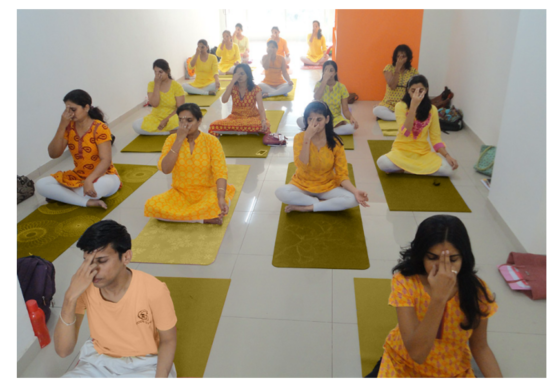
\includegraphics[width=\linewidth,keepaspectratio]{ycb1_teaching_demo}
		
		{\tiny (Ref: Certification  of Yoga Professionals Official Guidebook For Level I (Instructor))}		
        \end{center}	
    \end{column}
\end{columns}
\end{frame}


%%%%%%%%%%%%%%%%%%%%%%%%%%%%%%%%%%%%%%%%%%%%%%%%%%%%%%%%%%%%%%%%%%%%%%%%%%%%%%%%%%
\begin{frame}[fragile]\frametitle{}
\begin{center}
{\Large Principles  of  teaching  Yoga  protocol  to  different  groups  (beginners,  children,  youth, women, Geriatric population, and special attention group)}
\end{center}
\end{frame}

%%%%%%%%%%%%%%%%%%%%%%%%%%%%%%%%%%%%%%%%%%%%%%%%%%%%%%%%%%%
\begin{frame}[fragile]\frametitle{Principles of Teaching Yoga Protocol to Different Groups}
\begin{columns}
    \begin{column}[T]{0.5\linewidth}
      \begin{itemize}
        \item \textbf{Beginners}: Use \textbf{simple} instructions and \textbf{basic poses}.
        \item \textbf{Children}: Include \textbf{fun} and \textbf{interactive} elements.
        \item \textbf{Youth}: Emphasize \textbf{strength} and \textbf{endurance}.
        \item \textbf{Women}: Adapt for \textbf{pregnancy} and \textbf{menstruation}.
        \item \textbf{Geriatric Population}: Focus on \textbf{gentle} movements and \textbf{balance}.
        \item \textbf{Special Attention Group}: Customize for \textbf{health conditions} and \textbf{physical limitations}.
      \end{itemize}
    \end{column}
    \begin{column}[T]{0.5\linewidth}
        \begin{center}
        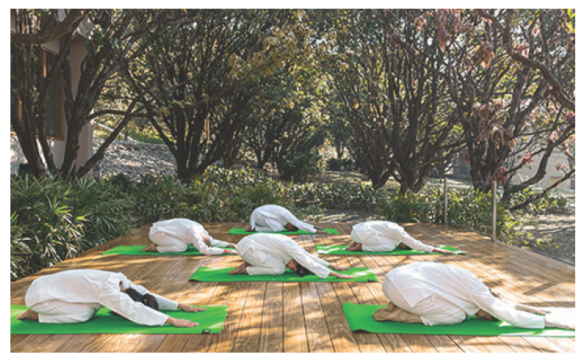
\includegraphics[width=\linewidth,keepaspectratio]{ycb1_teaching_group}
		
		{\tiny (Ref: Certification  of Yoga Professionals Official Guidebook For Level I (Instructor))}		
        \end{center}	
    \end{column}
\end{columns}
\end{frame}


%%%%%%%%%%%%%%%%%%%%%%%%%%%%%%%%%%%%%%%%%%%%%%%%%%%%%%%%%%%%%%%%%%%%%%%%%%%%%%%%%%
\begin{frame}[fragile]\frametitle{}
\begin{center}
{\Large Preparation for a Yoga class (before and during the class)}
\end{center}
\end{frame}

%%%%%%%%%%%%%%%%%%%%%%%%%%%%%%%%%%%%%%%%%%%%%%%%%%%%%%%%%%%
\begin{frame}[fragile]\frametitle{Preparation for a Yoga Class (Before and During)}
\begin{columns}
    \begin{column}[T]{0.5\linewidth}
      \begin{itemize}
        \item \textbf{Pre-Class Planning}: Develop a \textbf{lesson plan} and \textbf{set goals}.
        \item \textbf{Set Up Space}: Arrange \textbf{props} and \textbf{equipment} for \textbf{class}.
        \item \textbf{Check Equipment}: Ensure all \textbf{yoga mats} and \textbf{tools} are \textbf{clean} and \textbf{functional}.
        \item \textbf{Greet Students}: Welcome students and \textbf{address} any \textbf{individual needs}.
        \item \textbf{Monitor Flow}: Adjust the \textbf{class} as needed based on \textbf{student feedback} and \textbf{progress}.
      \end{itemize}
    \end{column}
    \begin{column}[T]{0.5\linewidth}
        \begin{center}
        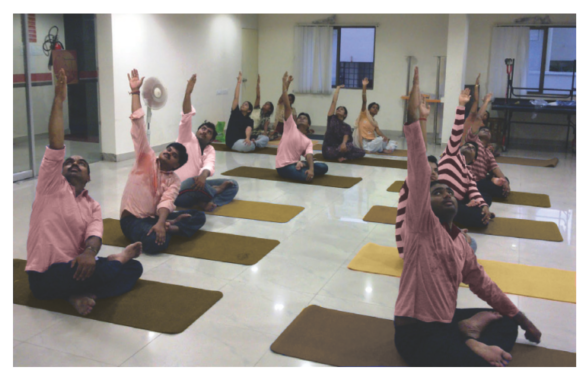
\includegraphics[width=\linewidth,keepaspectratio]{ycb1_teaching_prep}
		
		{\tiny (Ref: Certification  of Yoga Professionals Official Guidebook For Level I (Instructor))}	
        \end{center}	
    \end{column}
\end{columns}
\end{frame}


%%%%%%%%%%%%%%%%%%%%%%%%%%%%%%%%%%%%%%%%%%%%%%%%%%%%%%%%%%%%%%%%%%%%%%%%%%%%%%%%%%
\begin{frame}[fragile]\frametitle{}
\begin{center}
{\Large Conducting yoga practical lessons: Precautions \& Contraindications of practices}
\end{center}
\end{frame}

%%%%%%%%%%%%%%%%%%%%%%%%%%%%%%%%%%%%%%%%%%%%%%%%%%%%%%%%%%%
\begin{frame}[fragile]\frametitle{Conducting Yoga Practical Lessons: Precautions \& Contraindications}
\begin{columns}
    \begin{column}[T]{0.5\linewidth}
      \begin{itemize}
        \item \textbf{Assess Individual Needs}: Evaluate \textbf{health conditions} and \textbf{physical limitations}.
        \item \textbf{Modify Poses}: Adapt \textbf{asanas} to suit \textbf{individual needs}.
        \item \textbf{Monitor Students}: Watch for \textbf{discomfort} or \textbf{strain}.
        \item \textbf{Avoid Overexertion}: Prevent \textbf{overexertion} and \textbf{injuries}.
        \item \textbf{Educate on Contraindications}: Inform about \textbf{contraindications} for specific \textbf{conditions}.
      \end{itemize}
    \end{column}
    \begin{column}[T]{0.5\linewidth}
        \begin{center}
        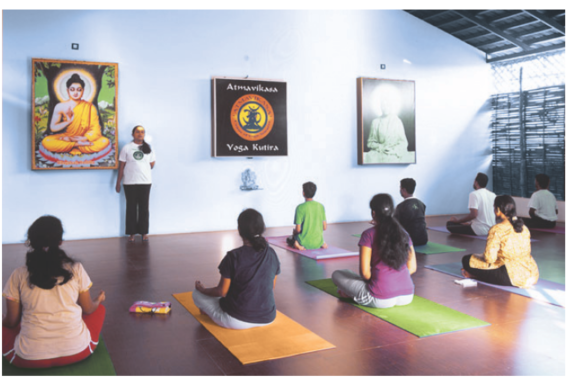
\includegraphics[width=\linewidth,keepaspectratio]{ycb1_teaching_lecture}
		
		{\tiny (Ref: Certification  of Yoga Professionals Official Guidebook For Level I (Instructor))}	
        \end{center}	
    \end{column}
\end{columns}
\end{frame}


%%%%%%%%%%%%%%%%%%%%%%%%%%%%%%%%%%%%%%%%%%%%%%%%%%%%%%%%%%%%%%%%%%%%%%%%%%%%%%%%%%
\begin{frame}[fragile]\frametitle{}
\begin{center}
{\Large Salient features of Ideal Yoga Instructor}
\end{center}
\end{frame}

%%%%%%%%%%%%%%%%%%%%%%%%%%%%%%%%%%%%%%%%%%%%%%%%%%%%%%%%%%%
\begin{frame}[fragile]\frametitle{Salient Features of an Ideal Yoga Instructor}
\begin{columns}
    \begin{column}[T]{0.5\linewidth}
      \begin{itemize}
        \item \textbf{Knowledgeable}: Deep understanding of \textbf{yoga principles} and \textbf{practices}.
        \item \textbf{Communicative}: Clear and \textbf{effective communication} skills.
        \item \textbf{Empathetic}: Ability to \textbf{understand} and \textbf{address student needs}.
        \item \textbf{Professional}: Maintains \textbf{professionalism} and \textbf{ethics}.
        \item \textbf{Adaptable}: Flexible in \textbf{teaching methods} and \textbf{lesson plans}.
      \end{itemize}
    \end{column}
    \begin{column}[T]{0.5\linewidth}
        \begin{center}
        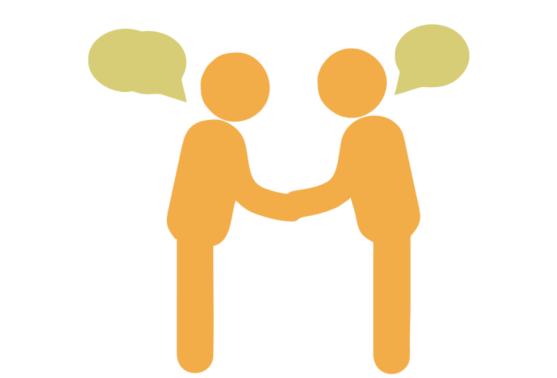
\includegraphics[width=\linewidth,keepaspectratio]{ycb1_teaching_teacher}
		
		{\tiny (Ref: Certification  of Yoga Professionals Official Guidebook For Level I (Instructor))}	
        \end{center}	
    \end{column}
\end{columns}
\end{frame}


%%%%%%%%%%%%%%%%%%%%%%%%%%%%%%%%%%%%%%%%%%%%%%%%%%%%%%%%%%%%%%%%%%%%%%%%%%%%%%%%%%
\begin{frame}[fragile]\frametitle{}
\begin{center}
{\Large Models of ideal Yoga lesson plans}
\end{center}
\end{frame}

%%%%%%%%%%%%%%%%%%%%%%%%%%%%%%%%%%%%%%%%%%%%%%%%%%%%%%%%%%%
\begin{frame}[fragile]\frametitle{Models of Ideal Yoga Lesson Plans}
\begin{columns}
    \begin{column}[T]{0.5\linewidth}
      \begin{itemize}
        \item \textbf{Structured Flow}: Follow a \textbf{logical sequence} of \textbf{warm-up}, \textbf{practice}, and \textbf{cool-down}.
        \item \textbf{Objective Focused}: Align \textbf{objectives} with \textbf{student needs} and \textbf{goals}.
        \item \textbf{Time Management}: Allocate \textbf{time} for each \textbf{segment} of the lesson.
        \item \textbf{Variety}: Incorporate a \textbf{variety} of \textbf{asanas}, \textbf{pranayama}, and \textbf{meditation}.
        \item \textbf{Flexibility}: Be \textbf{flexible} to \textbf{adapt} to \textbf{student feedback}.
      \end{itemize}
    \end{column}
    \begin{column}[T]{0.5\linewidth}
        \begin{center}
        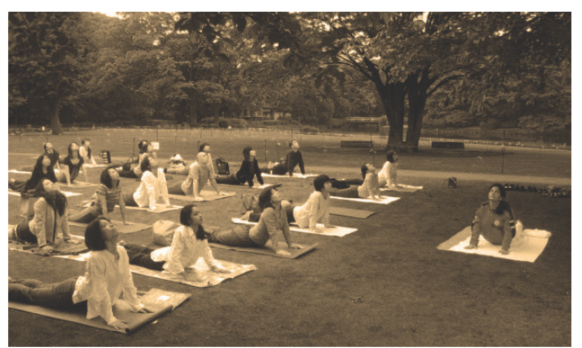
\includegraphics[width=\linewidth,keepaspectratio]{ycb1_teaching_lesson}
		
		{\tiny (Ref: Certification  of Yoga Professionals Official Guidebook For Level I (Instructor))}	
        \end{center}	
    \end{column}
\end{columns}
\end{frame}


%%%%%%%%%%%%%%%%%%%%%%%%%%%%%%%%%%%%%%%%%%%%%%%%%%%%%%%%%%%%%%%%%%%%%%%%%%%%%%%%%%
\begin{frame}[fragile]\frametitle{}
\begin{center}
{\Large Yogalaya class}
\end{center}
\end{frame}

%%%%%%%%%%%%%%%%%%%%%%%%%%%%%%%%%%%%%%%%%%%%%%%%%%%%%%%%%%%%%%%%%%%%%%%%%%%%%%%%%%
\begin{frame}[fragile]\frametitle{Starting Instructions and Initial Prayers}
\begin{itemize}
    \item Start Prayer
    \item Sit in comfortable sitting position, look straight
    \item Hands in Chin mudra, back straight, get ready for prayer
    \item Om, Om, Om
    \item गजाननं भूत गणादिसेवितं,
    \item कपीथ जम्बू फलचारु भक्षणं,
    \item गजाननं भूत गणादिसेवितं,
    \item कपीथ जम्बू फलचारु भक्षणं,
    \item उमासुतं शोक विनाश कारतम,
    \item नमामि विघ्नेशवर पादपंकजम,
    \item षडाननं कुम्कुमरक्तवर्णं
    \item महामतिं दिव्यमयूरवाहनम्
    \item रुद्रस्यसूनुं सुरसैन्यनाथं
    \item गुहं सदाहं शरणं प्रपद्ये
\end{itemize}
\end{frame}

%%%%%%%%%%%%%%%%%%%%%%%%%%%%%%%%%%%%%%%%%%%%%%%%%%%%%%%%%%%%%%%%%%%%%%%%%%%%%%%%%%
\begin{frame}[fragile]\frametitle{Continued Prayers}
\begin{itemize}
    \item या कुन्देन्दुतुषारहारधवला या शुभ्रवस्त्रावृता
    \item या वीणावरदण्डमण्डितकरा या श्वेतपद्मासना
    \item या ब्रह्माच्युतशंकरप्रभृतिभिर्देवै: सदा वन्दिता
    \item सा मां पातु सरस्वती भगवती नि:शेषजाड्यापहा
    \item ॐ नमः शिवाय गुरवे
    \item सच्चिदानन्द मूर्तये ।
    \item निष्प्रपञ्चाय शान्ताय
    \item (निरालम्बाय तेजसे ॥) 
    \item श्री शिवनंदाय तेनम:
    \item श्री विष्णू देवानंदाय तेनाम:
    \item सर्वमङ्गलमाङ्गल्ये शिवे सर्वार्थसाधिके ।
    \item शरण्ये त्र्यम्बके गौरि नारायणि नमोऽस्तु ते, नारायणि नमोऽस्तु ते
    \item ॐ सह नाववतु । सह नौ भुनक्तु । सह वीर्यं करवावहै ।
    \item तेजस्वि नावधीतमस्तु मा विद्विषावहै ।
    \item ॐ शान्तिः शान्तिः शान्तिः ॥
    \item ॐ नमः शिवाय ।।
\end{itemize}
\end{frame}

%%%%%%%%%%%%%%%%%%%%%%%%%%%%%%%%%%%%%%%%%%%%%%%%%%%%%%%%%%%%%%%%%%%%%%%%%%%%%%%%%%
\begin{frame}[fragile]\frametitle{Preparation for Pranayama}
\begin{itemize}
    \item Sit in comfortable sitting position, look straight
    \item Hands in Chin mudra, back straight, get ready for kapalbhati
    \item Inhale abdomen out, exhale in, inhale, exhale
    \item Now inhale deeply and begin
\end{itemize}
\end{frame}

%%%%%%%%%%%%%%%%%%%%%%%%%%%%%%%%%%%%%%%%%%%%%%%%%%%%%%%%%%%%%%%%%%%%%%%%%%%%%%%%%%
\begin{frame}[fragile]\frametitle{Kapalbhati Practice}
\begin{itemize}
    \item Exhale (20 times)
    \item Exhale (36 times)
    \item Exhale (5 times), inhale, exhale
    \item Now inhale deeply, comfortable breath and hold (20? seconds)
    \item With control, exhale, inhale, exhale
    \item Another round?
    \item Breathe normally, stretch legs, shake your legs and sit back again
\end{itemize}
\end{frame}

%%%%%%%%%%%%%%%%%%%%%%%%%%%%%%%%%%%%%%%%%%%%%%%%%%%%%%%%%%%%%%%%%%%%%%%%%%%%%%%%%%
\begin{frame}[fragile]\frametitle{Nadi Shodhana (Alternate Nostril Breathing)}
\begin{itemize}
    \item Left hand in chin mudra, right hand in vishnu mudra
    \item Inhale through both nostrils deeply
    \item Take your right thumb to right nostril, exhale through left nostril completely
    \item Inhale left 2-3-4 close, hold, close both nostrils, 8 sec?
    \item Exhale right 2-3-4-5-6-7-8, inhale right 2-3-4 close, hold
    \item Exhale left 2-3-4-5-6-7-8 Inhale left
    \item Repeat cycle
\end{itemize}
\end{frame}

%%%%%%%%%%%%%%%%%%%%%%%%%%%%%%%%%%%%%%%%%%%%%%%%%%%%%%%%%%%%%%%%%%%%%%%%%%%%%%%%%%
\begin{frame}[fragile]\frametitle{Post-Pranayama Meditation}
\begin{itemize}
    \item Drop your hands down, both hands in chin mudra, back straight
    \item Breathing comfortable
    \item Eyeball steady on one point, meditate, breathing relaxed
\end{itemize}
\end{frame}

%%%%%%%%%%%%%%%%%%%%%%%%%%%%%%%%%%%%%%%%%%%%%%%%%%%%%%%%%%%%%%%%%%%%%%%%%%%%%%%%%%
\begin{frame}[fragile]\frametitle{Shavasana and Concluding Stretch}
\begin{itemize}
    \item Release the mudra, stretch your legs and lie down in shavasana
    \item Feet apart, hands apart, palms facing upward
    \item Bring your feet together, inhale
    \item Bring your arms over and above your head, interlock fingers
    \item Turn your palms and stretch
    \item Exhale and release, bend your knees
    \item Turn to the right side, inhale and come up
\end{itemize}
\end{frame}

%%%%%%%%%%%%%%%%%%%%%%%%%%%%%%%%%%%%%%%%%%%%%%%%%%%%%%%%%%%%%%%%%%%%%%%%%%%%%%%%%%
\begin{frame}[fragile]\frametitle{Sun Salutations - First Round}
\begin{itemize}
    \item Stand in front of the mat, t-shirts tucked in. Stand straight
    \item Both hands in Namaskar position, near your chest
    \item Raise your arms up, arch back
    \item Bend forward and down
    \item Take your right leg back, knee down, toe pointing back, look up
    \item Left leg back, body into straight line
    \item Knees, chest, forehead or chin down
    \item Slide forward arch back
    \item Tuck your toes in, inverted V
    \item Take your right leg forward
    \item Left leg forward
    \item Raise your arms arch back and release
\end{itemize}
\end{frame}

%%%%%%%%%%%%%%%%%%%%%%%%%%%%%%%%%%%%%%%%%%%%%%%%%%%%%%%%%%%%%%%%%%%%%%%%%%%%%%%%%%
\begin{frame}[fragile]\frametitle{Sun Salutations - Second Round}
\begin{itemize}
    \item Feet together, palms together
    \item Raise your arms up, arch back
    \item Bend forward and down
    \item Take your left leg back, knee down, toe pointing back, look up
    \item Right leg back, body into straight line
    \item Knees, chest, forehead or chin down
    \item Slide forward arch back
    \item Tuck your toes in, inverted V
    \item Take your left leg forward
    \item Right leg forward
    \item Raise your arms up arch back and release
    \item Feet together, palms together
\end{itemize}
\end{frame}

%%%%%%%%%%%%%%%%%%%%%%%%%%%%%%%%%%%%%%%%%%%%%%%%%%%%%%%%%%%%%%%%%%%%%%%%%%%%%%%%%%
\begin{frame}[fragile]\frametitle{Sun Salutations with Breath Coordination - Right Side}
\begin{itemize}
    \item Inhale - exhale and palms together
    \item Inhale - Raise your arms up, arch back
    \item Exhale - Bend forward and down
    \item Inhale - right leg back
    \item Retain - other leg back
    \item Exhale - Knees, chest, forehead or chin down
    \item Inhale - Slide forward arch back
    \item Exhale - inverted V
    \item Inhale - right leg forward
    \item Exhale - left leg forward
    \item Inhale - Raise your arms up arch back
    \item Exhale - release
\end{itemize}
\end{frame}

%%%%%%%%%%%%%%%%%%%%%%%%%%%%%%%%%%%%%%%%%%%%%%%%%%%%%%%%%%%%%%%%%%%%%%%%%%%%%%%%%%
\begin{frame}[fragile]\frametitle{Sun Salutations with Breath Coordination - Left Side}
\begin{itemize}
    \item Inhale - exhale and palms together
    \item Inhale - Raise your arms up, arch back
    \item Exhale - Bend forward and down
    \item Inhale - left leg back
    \item Retain - other leg back
    \item Exhale - Knees, chest, forehead or chin down
    \item Inhale - Slide forward arch back
    \item Exhale - inverted V
    \item Inhale - left leg forward
    \item Exhale - right leg forward
    \item Inhale - Raise your arms up arch back
    \item Exhale - release
\end{itemize}
\end{frame}

%%%%%%%%%%%%%%%%%%%%%%%%%%%%%%%%%%%%%%%%%%%%%%%%%%%%%%%%%%%%%%%%%%%%%%%%%%%%%%%%%%
\begin{frame}[fragile]\frametitle{Cooling Down and Relaxation}
\begin{itemize}
    \item Feet apart, hands apart, palms facing forward
    \item Eyes closed, breathe through your nose
    \item Observe your heartbeats
    \item Observe your breathing
    \item Now lie down on your back and relax in shavasana
\end{itemize}
\end{frame}

%%%%%%%%%%%%%%%%%%%%%%%%%%%%%%%%%%%%%%%%%%%%%%%%%%%%%%%%%%%%%%%%%%%%%%%%%%%%%%%%%%
\begin{frame}[fragile]\frametitle{End Prayer}
\begin{itemize}
    \item Sit in comfortable sitting position, look straight
    \item Roll shoulders, hands in chin mudra
    \item Om, Om, Om
    \item ॐ पूर्णमद: पूर्णमिदं पूर्णात् , पूर्ण मुदच्यते, 
    \item पूर्णस्य पूर्णमादाय, पूर्ण मेवा वशिष्यते। 
    \item ॐ शांति: शांति: शांतिः
    \item सद्गुरू (?) शिवानंद महाराज कि जय, स्वामी विष्णू देवानंद महाराज कि जय 
    \item धर्मो रक्षति रक्षित: हरी ओम तत्सत 
    \item Rub hands, put palms on eyes and Namaskar!!
\end{itemize}
\end{frame}
